\chapter{System Development}
\label{chp:sys_dev}

\noindent In this Chapter, it will cover research about current \gls{webrtc} usage on real-time communication scenario and development progress of the prototype system along with explanation and analysis.

\section{WebRTC Current Usage}

\noindent In May 2011, Google released an open source project for browser-based real-time communication known as \gls{webrtc}. This has been followed by ongoing work to standardise the relevant protocols in the \gls{ietf} and browser \gls{api}s in the \gls{w3c}. Then more and more web application are using it in different ways. There are mainly two part of the \gls{webrtc} \gls{api}s could be used separately or cooperatively in the different web application.

\begin{itemize}[topsep=-1em,parsep=0em,itemsep=0em]
 \item \textbf{MediaStream:} get access to data streams, such as from the user's camera and microphone.
 \item \textbf{RTCPeerConnection:} audio or video calling, with facilities for encryption and bandwidth management.
 \item \textbf{RTCDataChannel:} peer-to-peer communication of generic data.
\end{itemize}

\par Because most of the application need to get the user's camera view and microphone sound, the \textit{MediaStream} \gls{api} is used always in real-time communication application. Normally \textit{MediaStream} \gls{api} will be used along with \textit{RTCPeerConnection} for showing remote peer media source content. The following business usage cases, 'Tropo' and 'Uberconference', are in this category.

\clearpage

\subsection{Tropo}

\par Tropo is an application platform that enables web developers to write communication applications in the languages they already use, Groovy\footnote{Groovy is an object-oriented programming language for the Java platform. It is a dynamic language with features similar to those of Python, Ruby, Perl, and Smalltalk.\cite{wiki:groovy}}, Ruby\footnote{Ruby is a dynamic, reflective, object-oriented, general-purpose programming language. It was designed and developed in the mid-1990s by Yukihiro "Matz" Matsumoto in Japan.\cite{wiki:ruby}}, \gls{php}\footnote{PHP is a server-side scripting language designed for web development but also used as a general-purpose programming language.\cite{wiki:php}}, Python\footnote{Python is a widely used general-purpose, high-level programming language.\cite{wiki:python}} and JavaScript\footnote{JavaScript (JS) is a dynamic computer programming language.\cite{wiki:js}}, or use a Web \gls{api} which will talk with an application running on your own server through the use of \gls{http} and \gls{json}, feeding requests and processing responses back and forth as needed. Tropo is in the cloud, so it manages the headaches of dealing with infrastructure and keeping applications up and running at enterprise-grade. With Tropo, developers can build and deploy voice and telephony applications, or add voice to existing applications.\cite{web:tropo}

\par It has some advanced features, like 'Phone numbers around the world', 'Text messaging', 'Transcription', 'Call Recording', 'Conferencing', 'Text to Speech' and 'Speech Recognition'. The prototype system in this thesis will provide similar functions like 'Text messaging' and 'Conferencing'. Since Tropo is a cloud application platform, it generates its own scripts based on programming language to provide developer possibility to easily use \gls{webrtc} to communicate with other kinds of network rather than \gls{ip} network. The functions Tropo provided is implemented in application server in the prototype, the application server will handle both the \gls{sip} stack and \gls{webrtc} stack in the system. For the client scripts will be host on the same application server for browser user to access and use.

\subsection{Uberconference}

\par UberConference fixes all the broken and outdated aspects of traditional conference calling, making it a more productive business tool, and transforming an industry that hasn't seen real innovation in decades. UberConference gives a visual interface to every conference call so callers can know who's on a call and who's speaking at any time, in addition to making many other features, such as Hangouts\footnote{Google Hangouts is an instant messaging and video chat platform developed by Google, which launched on May 15, 2013 during the keynote of its I/O development conference.\cite{wiki:hangouts}} integration and screen sharing, easy-to-use with the click of a button. Built by the teams that brought Google Voice\footnote{Google Voice (formerly GrandCentral) is a telecommunications service by Google launched on March 11, 2009.\cite{wiki:googleVoice}} and Yahoo! Voice to tens of millions of users, UberConference launched in 2012 and is funded by Andreessen Horowitz and Google Ventures.\cite{web:uberconference}

\begin{wrapfigure}{r}{0.6\textwidth}
	\centering
    	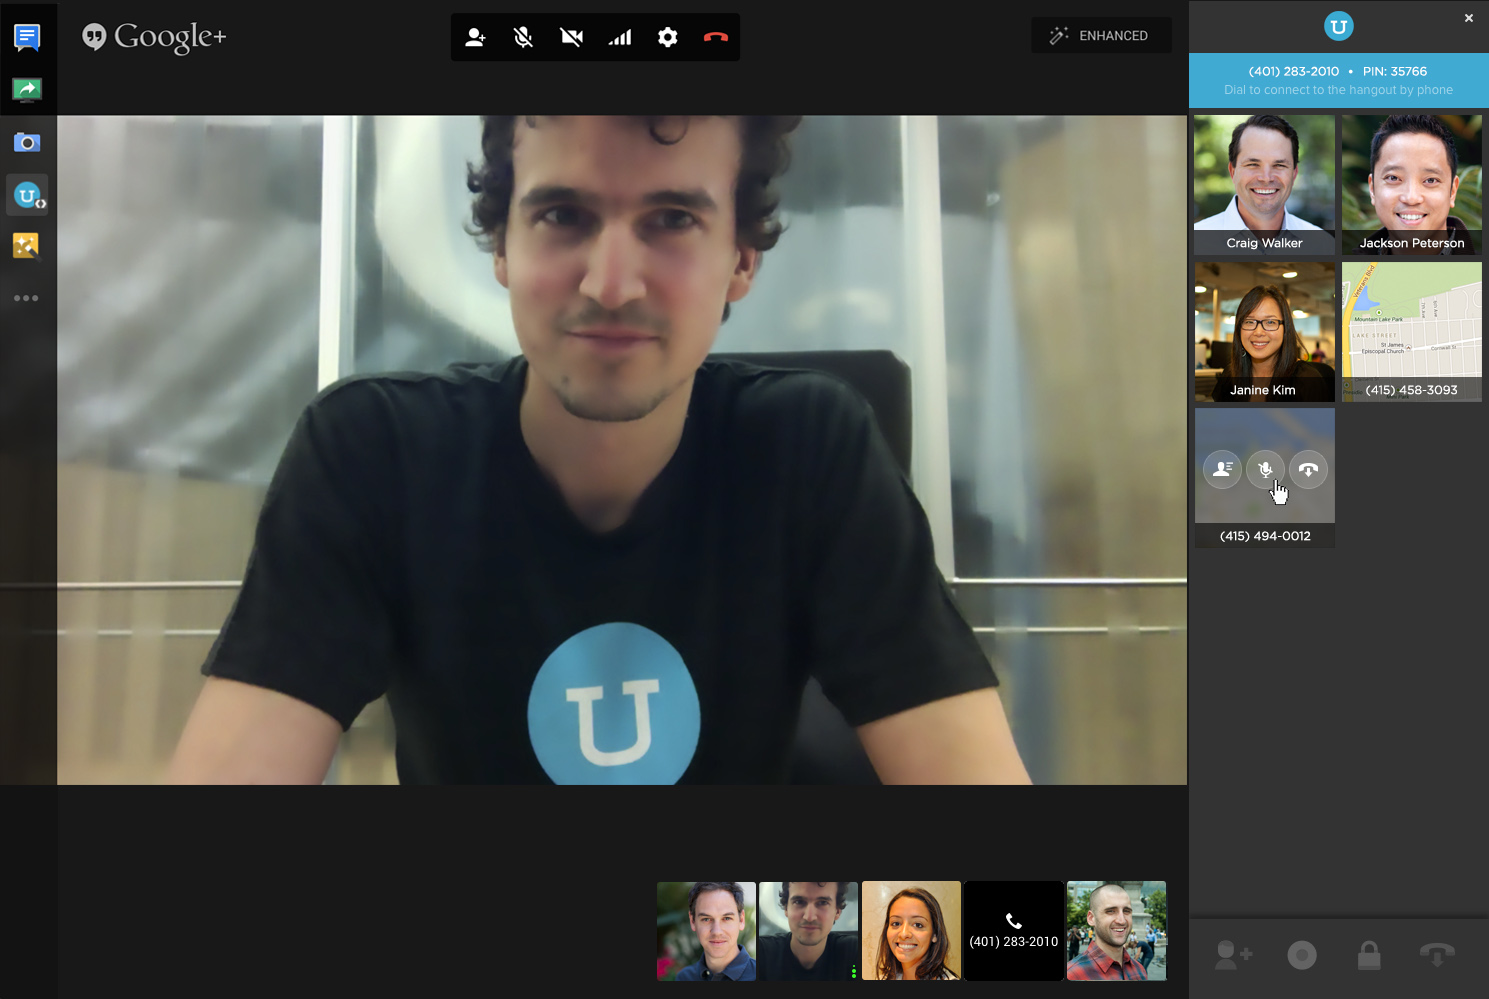
\includegraphics[width=0.58\textwidth,natwidth=610,natheight=642]{figs/uberconference_hangout.jpg}
  	\caption{UberConference integrate with Hangouts Screen shot\cite{tnw:uberconference}}
  	\label{fig:uberconference}
\end{wrapfigure}

\par The prototype system in this thesis is ideally to provide same rich media communication platform as the service provided by UberConference. In February of 2014, UberConference release the new feature which allow user to call into a Google Hangouts session with their mobile phone. The feature is shown in Figure \ref{fig:uberconference}, Once you have installed the UberConference app in Hangouts, people can join your call via phone with the help of a dedicated number. The prototype system will provide the same real-time communication service, but allow the user to use mobile phone number to create a video conference based on \gls{webrtc} on browser and communicate with audio only mobile phone user as well. It will be more easier for user since they just need to remember their user credential related to their mobile phone number to use the prototype application. During the real-time conversation, the prototype application will provide user cooperation tools like instance message and file sharing in this development phase.

\noindent However, there is another important \gls{api}, \textit{RTCDataChannel} , can be used more creatively by the developer to build web applications. The experiment  usage cases, 'Cube Slam' and 'Webtorrent', are in this category which is using \textit{RTCDataChannel} to build \gls{p2p} data sharing without data going though the server to dispatch to other peers. It works more efficiently to handle the synchronization problem.

\subsection{Cube Slam}

\par Cube Slam (shown in Figure \ref{fig:cube_slam}) is a Chrome Experiment built with \gls{webrtc} , play an old-school arcade game with your friends without downloading and installing any plug-ins. Cube Slam uses \textit{getUserMedia} to access user's webcam and microphone ,\textit{RTCPeerConnection} to stream user video to another user, and \textit{RTCDataChannel} to transfer the bits that keep the gameplay in sync. If two users are behind firewalls, \textit{RTCPeerConnection} uses a TURN  relay server (hosted on Google Compute Engine) to make the connection. However, when there are no firewalls in the way, the entire game happens directly peer-to-peer, reducing latency for players and server costs for developers.\cite{chrome:cube_slam}

\begin{figure}
	\centering
    	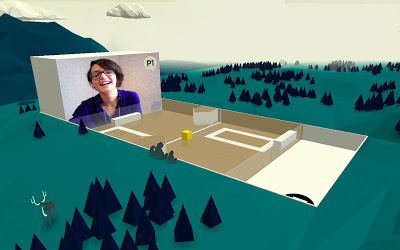
\includegraphics[width=0.8\textwidth,natwidth=610,natheight=642]{figs/cube_slam.jpg}
  	\caption{Cube Slam Game Over Screen}
  	\label{fig:cube_slam}
\end{figure}

\par The idea behind the Cube Slam is that use \textit{RTCDataChannel} to sync the player data in real-time to reduce the latency by peer to peer. \textit{RTCDataChannel} sends data securely, and supports an "unreliable" mode for cases where you want high performance but don't care about every single packet making it across the network. In cases like games where low delay often matters more than perfect delivery, this ensures that a single stray packet doesn't slow down the whole app. The prototype application in this thesis will still use WebSocket for data sharing instead of \textit{RTCDataChannel} because the media server using in this system is not support \textit{RTCDataChannel} yet, so it is not possible to create peer to peer session regarding to this issue. This case about \textit{RTCDataChannel} will be discussed in Chapter \ref{chp:future_work}.

\subsection{Webtorrent}


\section{WebRTC Implementation APIs}

\par In order to obtain local media, the \gls{webrtc} \gls{api}s provide \textit{getUserMedia()} function to get the video and audio stream from user. For privacy reasons, a web application’s request for access to a user’s microphone or camera will only be granted after the browser has obtained permission from the user. \textit{getUserMedia()} function is currently available in Chrome, Opera and Firefox. Almost all of the \gls{webrtc} \gls{api}s are slightly different in different browsers.

%% TODO: differences handling in different browsers

However, since \gls{webrtc} \gls{api}s is not standard \gls{api} yet, the prototype application in this thesis will not pay too much work-load on compatibility for different browsers platform.

\par For setting up peer connection, the core of \gls{webrtc} is the \textit{RTCPeerConnection} \gls{api}, which sets up a connection between two peers. In this context, “peers” means two communication endpoints on the World Wide Web. Instead of requiring communication through a server, the communication is direct between the two entities. In the specific case of \gls{webrtc}, a peer connection is a direct media connection between two web browsers. This is particularly relevant when a multi-way communication such as a conference call is set up among three or more browsers. Each pair of browsers will require a single peer connection to join them, allowing for audio and video media to flow directly between the two peers. 

%% TODO: Explaination for system architecture
%% The system architecture regarding to this \gls{webrtc} factor will be discussed in later Chapter \ref{chp:sys_dev} since there is consideration between centralized media server network and mesh network architecture.

\begin{figure}
	\centering
    	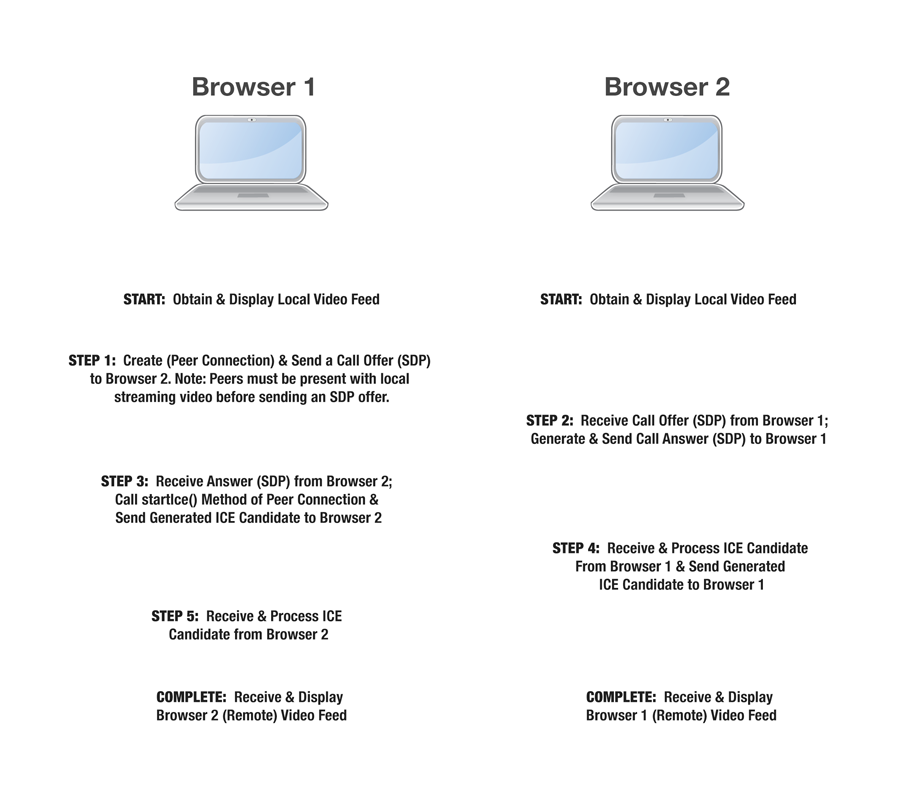
\includegraphics[height=0.50\textheight,natwidth=610,natheight=642]{figs/webrtc_diagram.png}
  	\caption{WebRTC Set up a call Process}
  	\label{fig:webrtc_diagram}
\end{figure}

\par To establish this connection requires a new \textit{RTCPeerConnection} object. The only input to the \textit{RTCPeerConnection} constructor method is a configuration object containing the information that \gls{ice}, will use to “punch holes” through intervening \gls{nat} devices and firewalls. There are two \gls{api}s to handle the  \textit{IceCandidate} object which contains \gls{ice} information data. One is \textit{onicecandidate} listener to trigger the function to handle the new \textit{IceCandidate} data object. The other one is \textit{addIceCandidate} function to add the new \textit{IceCandidate} data object to the remote/local peer connection session description field.

\par Once the \textit{RTCPeerConnection} is established, the client need configure where the media or data to store and display if it is necessary. In the prototype application of this thesis, media stream will be displayed in a \gls{html5} tag called \textit{<video>}. It will only be shown when there is media stream in \textit{<video>} tag source.

\par In order to make the \gls{webrtc} \gls{stun} server or \gls{turn} server to generate the \gls{ice} candidate for the peer client, the caller \textit{RTCPeerConnection} need run \textit{createOffer()} function and the callee need run \textit{createAnswer()} function  to ask the \gls{stun}/\gls{turn} server to find the path for each other peer.There is one calling process shown in Figure\ref{fig:webrtc_diagram}, it is a set up call process from caller peer.

\par \gls{webrtc} clients (known as peers) also need to ascertain and exchange local and remote audio and video media information, such as resolution and codec capabilities. Signaling to exchange media configuration information proceeds by exchanging an offer and an answer using the \gls{sdp}. The \textit{createOffer()} function and \textit{createAnswer()} function both have callback function to handle the \gls{sdp} either to call \textit{setLocalDescription()} by caller or call \textit{setRemoteDescription()} by callee when callee gets the caller's \gls{sdp} from \gls{webrtc} offer. The Log Snippet\ref{log:webrtc_answer_sdp} shown is the \gls{webrtc} answer \gls{sdp} from the callee when the callee end-point decide to accept this conversion session.

\begin{algorithm}[h]
\floatname{algorithm}{Log Snippet}
  \caption{Sample \gls{webrtc} Answer \gls{sdp}}
  \label{log:webrtc_answer_sdp}
  \begin{verbatim}
sdp: v=0
o=xmserver 1399363527 1399363528 IN IP4 10.254.9.135
s=xmserver
c=IN IP4 10.254.9.135
t=0 0
a=ice-lite
m=audio 49152 RTP/SAVPF 0 126
a=rtpmap:0 PCMU/8000
a=sendrecv
a=rtcp:49153
a=candidate:1 1 UDP 2130706431 10.254.9.135 49152 typ host
a=candidate:1 2 UDP 2130706430 10.254.9.135 49153 typ host
...
a=acfg:1 t=1
a=rtpmap:126 telephone-event/8000
a=fmtp:126 0-15
m=video 57344 RTP/SAVPF 100
b=AS:1000
a=rtpmap:100 VP8/90000
a=fmtp:100 max-fr=30; max-fs=1200
a=sendrecv
a=rtcp:57345
a=rtcp-fb:100 ccm fir
a=rtcp-fb:100 nack
a=rtcp-fb:100 nack pli
a=rtcp-fb:100 goog-remb
a=candidate:2 1 UDP 2130706431 10.254.9.135 57344 typ host
a=candidate:2 2 UDP 2130706430 10.254.9.135 57345 typ host
...
 \end{verbatim}
\end{algorithm}
